\documentclass[parskip,10pt,abstracton]{scrartcl}
\usepackage[top=3cm, bottom=3cm, left=3cm, right=3cm]{geometry}
\usepackage{polyglossia}
\setmainlanguage{german}
%\pagenumbering{gobble}

\usepackage{setspace}
\onehalfspacing

% ------------------------------------------------------------------------------------
% packages
\usepackage[hidelinks]{hyperref}
\usepackage{graphicx}
\usepackage{tikz}
\usetikzlibrary{arrows,shapes,positioning, shadows,trees}
\usepackage{enumerate}

\usepackage{xcolor}
\usepackage{pdfpages}
\newcommand{\sbt}{\begin{picture}(-1,1)(-1,-3)\circle*{3}\end{picture}\ } % Punkt


% ------------------------------------------------------------------------------------
% Header
% ------------------------------------------------------------------------------------
\renewcommand*{\maketitle}{%
	\begin{flushright}
	{\rmfamily WiSe 16/17 \par}
	\end{flushright}
	\vspace{-1.3cm}
	
	{\bfseries\sffamily User-Interface Design} \\
	{\rmfamily Tamar Arndt \\ Jens-Christan Foerster \\ Velat Gümüs \par}
	
	{\centering\LARGE\sffamily\bfseries Nutzertest \par}
	\vspace{1em}
}

%\renewcommand{\thesection}{}
% ====================================================================================
% Document
% ====================================================================================
\begin{document}

\maketitle

%\tableofcontents


% ------------------------------------------------------------------------------------
% AUFGABE 9
% ------------------------------------------------------------------------------------
\section*{Protokolle} 
\textbf{Durchführung}\\
\begin{appendix}
%\addcontentsline{toc}{section}{Anhang}
\textcolor{teal}{Versuchsleiter: Velat | Protokollant: Chris}\\
\textcolor{teal}{Probandennummer: 1 | Alter: 27 | Internetnutzung: 4}

\textcolor{gray}{
Danke, dass du dir die Zeit nimmst, unsere Webseite zu testen. 
Wir wollen unsere Webseite von Nutzern testen lassen, um mögliche Fehler zu identifizieren und ggf. zu beheben. \\
Zum Ablauf: Der Nutzertest besteht zum einen aus drei Aufgaben und zum anderen einen Fragebogen. Versuche während der Bearbeitung der Aufgaben "laut zu denken", damit wir deine Gedanken protokollieren können. D.h. du musst aussprechen, was du denkst, was du siehst und worin du gerade Schwierigkeiten hast. 
}\\\\
\textcolor{gray}{
\textbf{Aufgabe 1:} Wähle das Gericht „indischer Pilaw“ aus und füge es zu deinem Kochbuch hinzu. Dafür musst du dich vorher einloggen. Logge dich anschließend wieder aus.}

\textit{Also als erstes muss ich mich einloggen. Das muss eigentlich auf der rechten oberen Seite sein, sowie überall auch. Okay, ich logge mich einfach mit den gegebenen Daten ein. So, jetzt muss ich das Gericht finden. Ich weiß nicht was "Pilaw" ist, deshalb muss ich mal mit der Maus überall drüber gehen. Das zweite Gericht ist ja schon der indische Pilaw. Dann klicke ich mal das Rezept an und hier wahrscheinlich auf "Rezept merken", denke ich mal. Okay, das wurde also jetzt meinem persönlichen Kochbuch hinzugefügt, sowie es hier steht. Und jetzt logge ich mich auch rechts oben wieder aus.}\\
\textcolor{teal}{Dauer: 33 sec, Mausklicks: 5, Erfolg: ja}\\\\

\textcolor{gray}{
\textbf{Aufgabe 2:} Suche nach Rezepten mit Gemüse. Wähle eines aus und finde heraus, wie es zubereitet wird und ob es kompliziert zuzubereiten ist.}\\
\textit{Also vermutlich muss ich ich diesen Filter auf der linken Seite benutzen. Gerichte mit Gemüse sind doch vegetarisch oder so... Also muss ich ja unter Ernährungsweise nachsehen. Doch nicht, hier im Suchfeld steht ja bereits Gemüse drin. Ich muss wahrscheinlich hier danach suchen. Na wer sagt's denn? Rucolasalat hört sich lecker an... Und wie es aussieht, ist es auch einfach zuzubereiten.}\\
\textcolor{teal}{Dauer: 44 sec, Mausklicks: 5, Erfolg: ja}\\\\

\textcolor{gray}{
\textbf{Aufgabe 3:} Filtere die Gerichte nach den Stichworten „Mittag“ und „vegetarisch“. Wähle den „Rucolasalat“ aus und finde heraus, wie er zubereitet wird. Setze anschließend die Auswahl wieder zurück.}

\textit{Also das muss ich auf jeden Fall hier auf der linken Seite machen. Also Mittag habe ich jetzt ausgewählt und vegetarisch ist ja hier unten. So, den Rucolasalat kenne ich ja bereits. Ich weiß ja auch, dass er einfach zuzubereiten ist. Also kann ich jetzt da oben die Auswahl wieder zurücksetzen. }\\
\textcolor{teal}{Dauer: 33 sec, Mausklicks: 7, Erfolg: ja}
%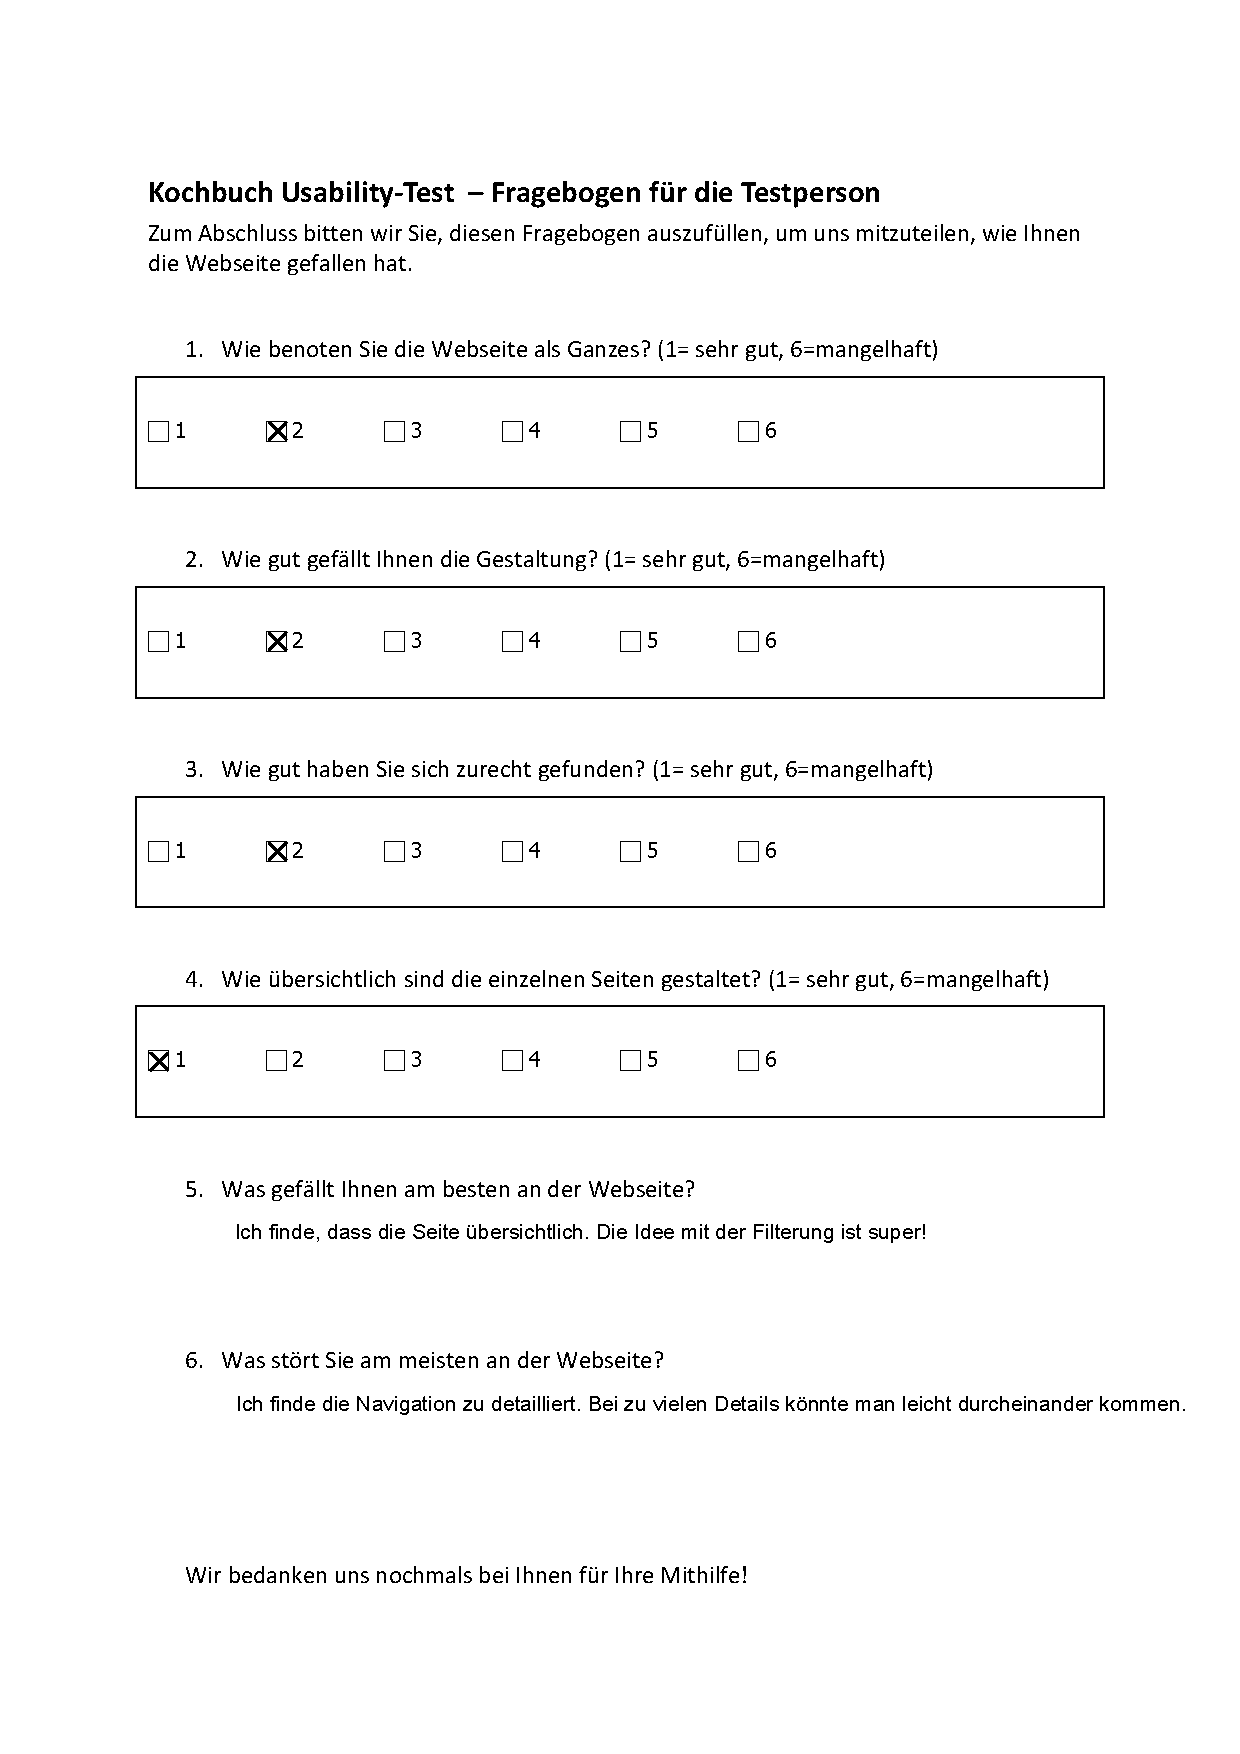
\includepdf[pages=-, scale=0.8]{Fragebogen_Proband1.pdf}
%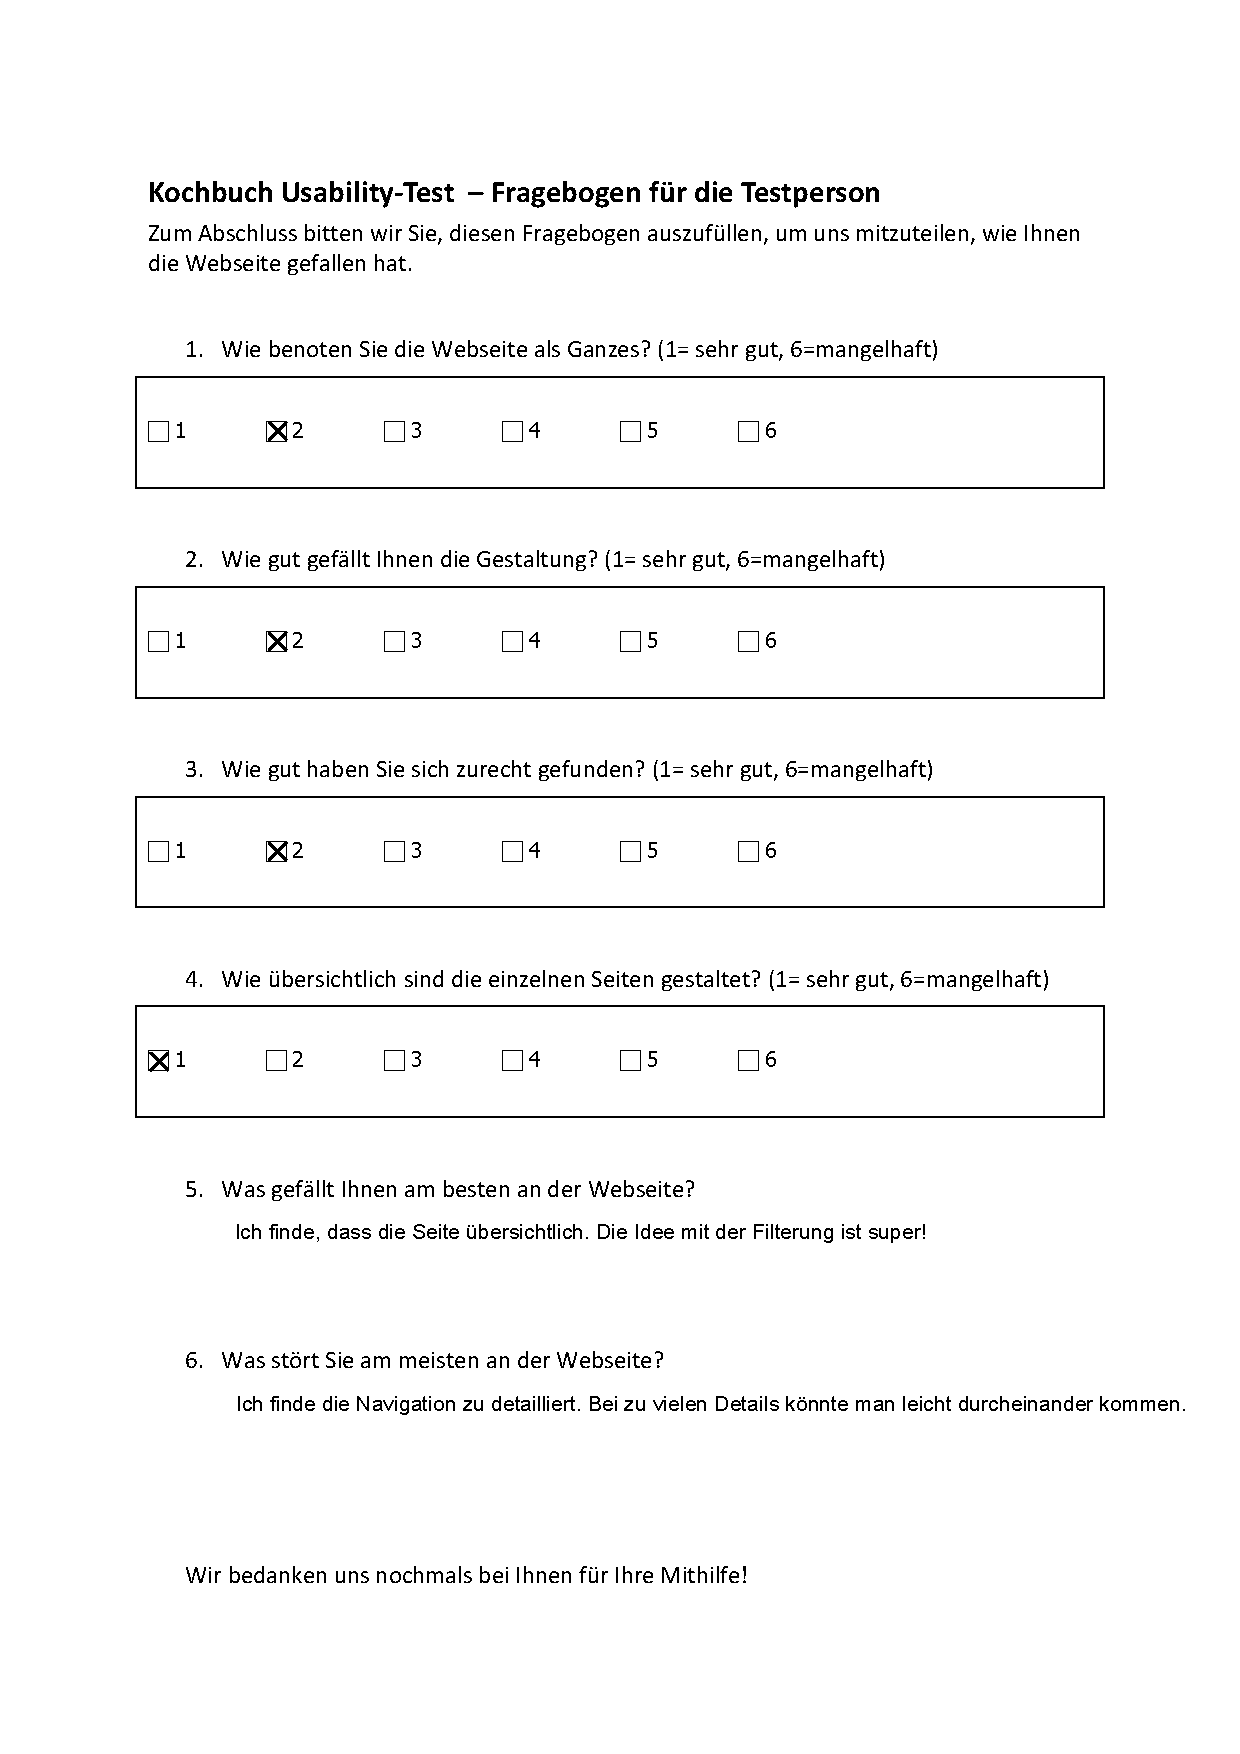
\includegraphics[width=0.8\textwidth]{Fragebogen_Proband1.pdf}
\newpage
\textcolor{teal}{Versuchsleiter: Chris | Protokollantin: Tamar}\\
\textcolor{teal}{Probandennummer: 2 | Alter: 24 | Internetnutzung: 4}

\textcolor{gray}{
Vielen Dank, dass du bei unserem Nutzertest mitmachst.
Zuerst ein paar Informationen: Wir möchten dir gerne die Webseite, an der wir arbeiten zeigen und sehen ob alles gut funktioniert und für dich angenehm zu benutzen ist.
Es dauert ungefähr 10 Minuten. \\
Ich gebe dir gleich 3 kurze Aufgaben und zeige dir die Webseite.
Bitte versuche dabei, deine Gedanken laut auszusprechen. Erzähle einfach, was du siehst, was du gerade tust und was du denkst. Ich werde neben dir sitzen und protokollieren.
Hast du bis hierher Fragen?
}

\textcolor{gray}{
Gut, dann zeige ich dir jetzt die Webseite. Bitte sieh sie dir ersteinmal an. Klicke noch nichts an und erzähle mir was du denkst.
}

\textit{Ah, ein Kochbuch also. Der rote Button dort rechts ist ein bisschen komisch. Warum ist der nicht ganz rechts am Rand? Und wenn es ein Button ist, könnte er auch einen Schatten haben - wie der hier drüben.} [scrollt] \textit{Aber insgesamt, sieht es ganz nett aus.}

\textcolor{gray}{
Okay, danke, dann gebe ich dir als Nächstes 3 Aufgaben nacheinander. Bitte versuche diese mit der Webseite zu bearbeiten. Wenn du etwas nicht direkt finden kannst, dann ist das kein Problem. Du kannst hier nichts falsch machen. Bitte versuche so viel wie möglich deine Gedanken dabei auszusprechen.}\\

\textcolor{gray}{
\textbf{Aufgabe 1:} Wähle das Gericht „indischer Pilaw“ aus und füge es zu deinem Kochbuch hinzu. Dafür musst du dich vorher einloggen. Logge dich anschließend wieder aus.}

\textit{Hier auf der Startseite sehe ich den indischen Pilaw. Aber ich muss mich ja erst einloggen. Dann klicke ich jetzt auf „mein Kochbuch“ und auf Login. Ich nehme die vorgeschlagenen Logindaten und logge mich ein. Ach, ich habe schon einige Rezepte gespeichert. Da ist schon der Pilaw. Mh. Ich klicke trotzdem nochmal drauf. Jetzt klicke ich auf „Rezept merken“. Und bekomme eine Rückmeldung, dass es hinzugefügt wurde. Das ist nett. Jetzt ist das Rezept immer noch bei meinen Rezepten ;). Jetzt logge ich mich bei „mein Kochbuch“ unten wieder aus. Ach, dafür bekomme ich auch eine Meldung.}\\
\textcolor{teal}{Dauer: 36 sec, Mausklicks: 5, Erfolg: ja}\\


\textcolor{gray}{
\textbf{Aufgabe 2:} Suche nach Rezepten mit Gemüse. Wähle eines aus und finde heraus, wie es zubereitet wird und ob es kompliziert zuzubereiten ist.}

\textit{Auf der rechten Seite ist ja alles, was ich gebrauchen kann. Das Suchfeld habe ich vorhin schon gesehen. Mh. ich lese die Notiz darunter - na, das hätte ich mir auch so gedacht. Also gebe ich „Gemüse“ ein und klicke Enter. Schön, dass das mit der Enter-Taste funktioniert. Das mit dem Bacon sieht gut aus. „gebratener Spargel“ - das nehme ich. Es ist mittelschwer zuzubereiten und hier sehe ich, wie ich es zubereiten muss. Hier bei dem vierten Schritt fehlt der Punkt. Aber es ist recht übersichtlich.}\\
\textcolor{teal}{Dauer: 28 sec, Mausklicks: 2, Erfolg: ja}\\


\textcolor{gray}{
\textbf{Aufgabe 3:} Filtere die Gerichte nach den Stichworten „Mittag“ und „vegetarisch“. Wähle den „Rucolasalat“ aus und finde heraus, wie er zubereitet wird. Setze anschließend die Auswahl wieder zurück.}

\textit{Dann gehe ich erstmal wieder auf die Startseite. Schade, dass man nicht hier oben auf das Logo klicken kann. Ich muss wohl auf „Auswahl zurücksetzen“... Ach da unten kann man filtern. Ich suche die Stichworte. Was waren die nochmal? Ach, dort ist „Mittag \& Abend“. Dann nehme ich das. Und klicke auf „filtern“. Ich klicke auf „Rucolasalat“ und kann lesen, wie er zubereitet wird. Mh mit Pilzen. Den Button „Auswahl zurücksetzen“ kenne ich ja schon. Jetzt bin ich wieder auf der Startseite.}\\
\textcolor{teal}{Dauer: 54 sec, Mausklicks: 10, Erfolg: ja}

%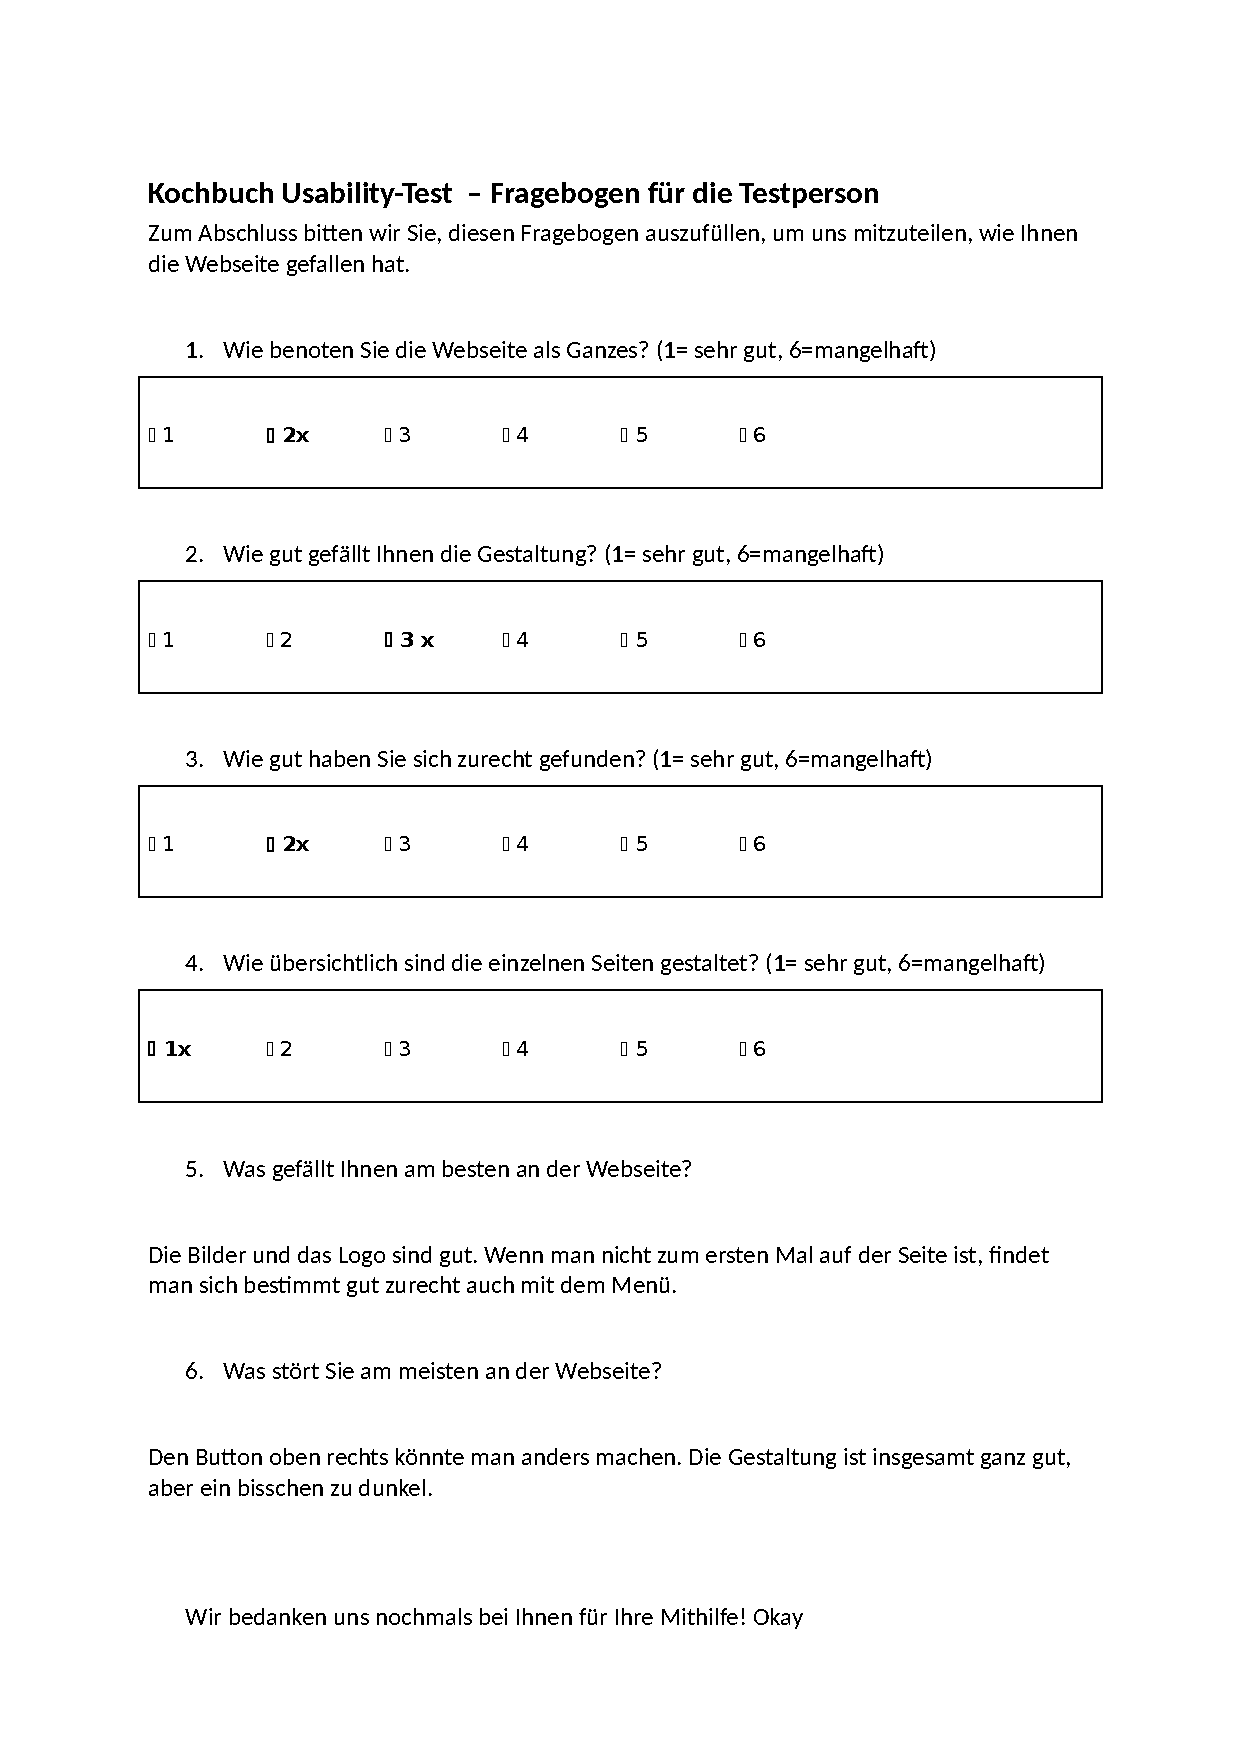
\includegraphics[width=0.8\textwidth]{Fragebogen_Proband2.pdf}
\newpage
\textcolor{teal}{Versuchsleiterin: Tamar | Protokollant: Velat}\\
\textcolor{teal}{Probandennummer: 3 | Alter: 21 | Internetnutzung: 4}

\textcolor{gray}{
Vielen Dank, dass du bei unserem Nutzertest mitmachst.
Zuerst ein paar Informationen: Wir möchten dir gerne die Webseite, an der wir arbeiten zeigen und sehen ob alles gut funktioniert und für dich angenehm zu benutzen ist.
Es dauert ungefähr 10 Minuten. \\
Ich gebe dir gleich 3 kurze Aufgaben und zeige dir die Webseite.
Bitte versuche dabei, deine Gedanken laut auszusprechen. Erzähle einfach, was du siehst, was du gerade tust und was du denkst. Ich werde neben dir sitzen und protokollieren.
Hast du bis hierher Fragen?
}

\textcolor{gray}{
Gut, dann zeige ich dir jetzt die Webseite. Bitte sieh sie dir ersteinmal an. Klicke noch nichts an und erzähle mir was du denkst.
}

\textit{
Das Logo ist hübsch. Die Farben auch. Aber das grün ist zu dunkel. Oder der Hintergrund? Alles ein bisschen zu dunkel vielleicht.} [liest den Willkommenstext] \textit{Warum ist dort ein Komma? und dann fängt es groß wieder an... Die Rezeptbilder sehen gut aus. Da drüben ist so eine Art Menü. Suchen... Filtern... aha. Der rote Button oben rechts ist komisch. Aber vielleicht soll das ja so sein. Die grünen Rezeptdinger sind irritierend. „placeholder“. naja, ihr hab ja nicht so viele Rezepte, deshalb ist das ganz gut, dass ihr die habt.} [sieht sich Rezeptbilder an, scrollt...]

\textcolor{gray}{
Okay, danke, dann gebe ich dir als Nächstes 3 Aufgaben nacheinander. Bitte versuche diese mit der Webseite zu bearbeiten. Wenn du etwas nicht direkt finden kannst, dann ist das kein Problem. Du kannst hier nichts falsch machen. Bitte versuche so viel wie möglich deine Gedanken dabei auszusprechen.}\\

\textcolor{gray}{
\textbf{Aufgabe 1:} Wähle das Gericht „indischer Pilaw“ aus und füge es zu deinem Kochbuch hinzu. Dafür musst du dich vorher einloggen. Logge dich anschließend wieder aus.}

\textit{
„Indischer Pilaw“. Weiß ja gar nicht, wie so etwas aussieht. Aber man sieht ja die Namen der Rezept. Oder soll ich lieber danach Suchen? ... Nein, hier ist das Rezept. Es sind ja nicht so viele, da findet man es auch so. ;)} [klickt auf das Rezept], \textit{Achso ich sollte mich einloggen. Aber ich kann ja trotzdem auf Rezept merken klicken. Na gut. Ich muss mich einloggen. Das geht bestimmt bei „mein Kochbuch“, da oben. Ja. Dann gebe ich da jetzt irgendetwas ein. Ich hoffe, es ist nicht wichtig, was genau.} [tippt irgendwas ein, klickt auf login, loginseite wird neu geladen] \textit{Das hat nicht funktioniert? Ich probiere es nochmal... ne... Ist das ein bug? Ich klicke einfach mal so auf Login. Mh das geht. Das müsst ihr nochmal überarbeiten} [Anmerkung: es geht wenn man in nur eines der Felder etwas eingibt. Verstehe selbst nicht, warum es nicht funktioniert wenn man jeweils etwas eintippt] \textit{Jetzt bin ich eingeloggt. Da ist das Rezept wieder. Ich klicke also drauf... und bin wieder auf der Seite. Mal sehen ob der Button jetzt funktionier. Ja. schön. Aber das Einloggen war komisch. An der Seite ändert sich auch gar nicht viel, wenn man jetzt eingeloggt ist. Was soll ich jetzt tun? Mich wieder ausloggen? Achso. Das Menü hat sich geändert. Dann klicke ich jetzt auf ausloggen. Fertig.}\\
\textcolor{teal}{Dauer: 69 sec, Mausklicks: 13, Erfolg: ja}\\


\textcolor{gray}{
\textbf{Aufgabe 2:} Suche nach Rezepten mit Gemüse. Wähle eines aus und finde heraus, wie es zubereitet wird und ob es kompliziert zuzubereiten ist.}

\textit{Suuchen... Hier drüben kann ich suchen. Da steht ja schon Gemüse. Vielleicht kann ich das einfach so lassen, wie vorhin bei dem Login. Ich gebe es trotzdem nochmal ein. Das geht. Das sind ja nicht viele Rezepte. Das sieht gut aus.} [klickt auf „Griechischer Brotsalat“] \textit{Mmh. Viele Zutaten. Sieht aber schön ordentlich aus mit den weißen Linien. Hier steht die Zubereitung. Das muss ich jezt aber nicht alles vorlesen, oder? ... So. Ausloggen muss ich mich diesmal nicht...}\\
\textcolor{teal}{Dauer: 30 sec, Mausklicks: 2, Erfolg: ja}\\


\textcolor{gray}{
\textbf{Aufgabe 3:} Filtere die Gerichte nach den Stichworten „Mittag“ und „vegetarisch“. Wähle den „Rucolasalat“ aus und finde heraus, wie er zubereitet wird. Setze anschließend die Auswahl wieder zurück.}

\textit{Dachte mir schon, dass ich als nächstes das mit dem Filtern machen soll... Hier oben kann ich noch irgendwas mit dem Suchbereich machen. Das habe ich auch noch nicht verwendet. Naja egal. Da unten ist der Button zum Filtern... den habe ich nicht sofort gesehen. Ist zu weit unten. Okay. hier gibt es „Zubereitungsart, Hauptzutat, Anlass“ - was soll Anlass heißen? „Land, Ernährungsweise...“ mh. Was soll ich nehmen? Achja Mittag... Ich klicke einfach mal alles an. Oh das ist ja blöd, dass die Seite immer hoch springt. Aber immerhin bleiben die Dinger ausgeklappt. Okay. Ach hier ist „Mittag \& Abend“. Passt das? Ich sehe nichts anderes zumindest. dann nehme ich das mal. Und vegetarisch kann ja nur unter Ernährungsweise sein. ... mh nochmal scrollen. ja hier. so. dann klicke ich jetzt auch Rezept filtern. Das geht. Die Nudeln sehen lecker aus! Aber ich soll ja Rucolasalat finden. Rucolasalat.. Rucolasalat.. Wenn es mehr Rezepte wären wäre es sicher ein bisschen nervig, überall drüber hovern zu müssen. Hier. Rucolasalat. Das Bild ist ein bisschen unscharf, oder? Naja. Aber hier steht die Zubereitung... Jetzt soll ich die Auswahl zurücksetzen. Das ist der Button da oben. Achso. „zurück zur Auswahl“ oder „Auswahl zurücksetzen“? Ist vielleicht egal. Ich nehme den Grünen. So. bin ich wieder auf der Startseite.}\\
\textcolor{teal}{Dauer: 80 sec, Mausklicks: 9, Erfolg: ja}

%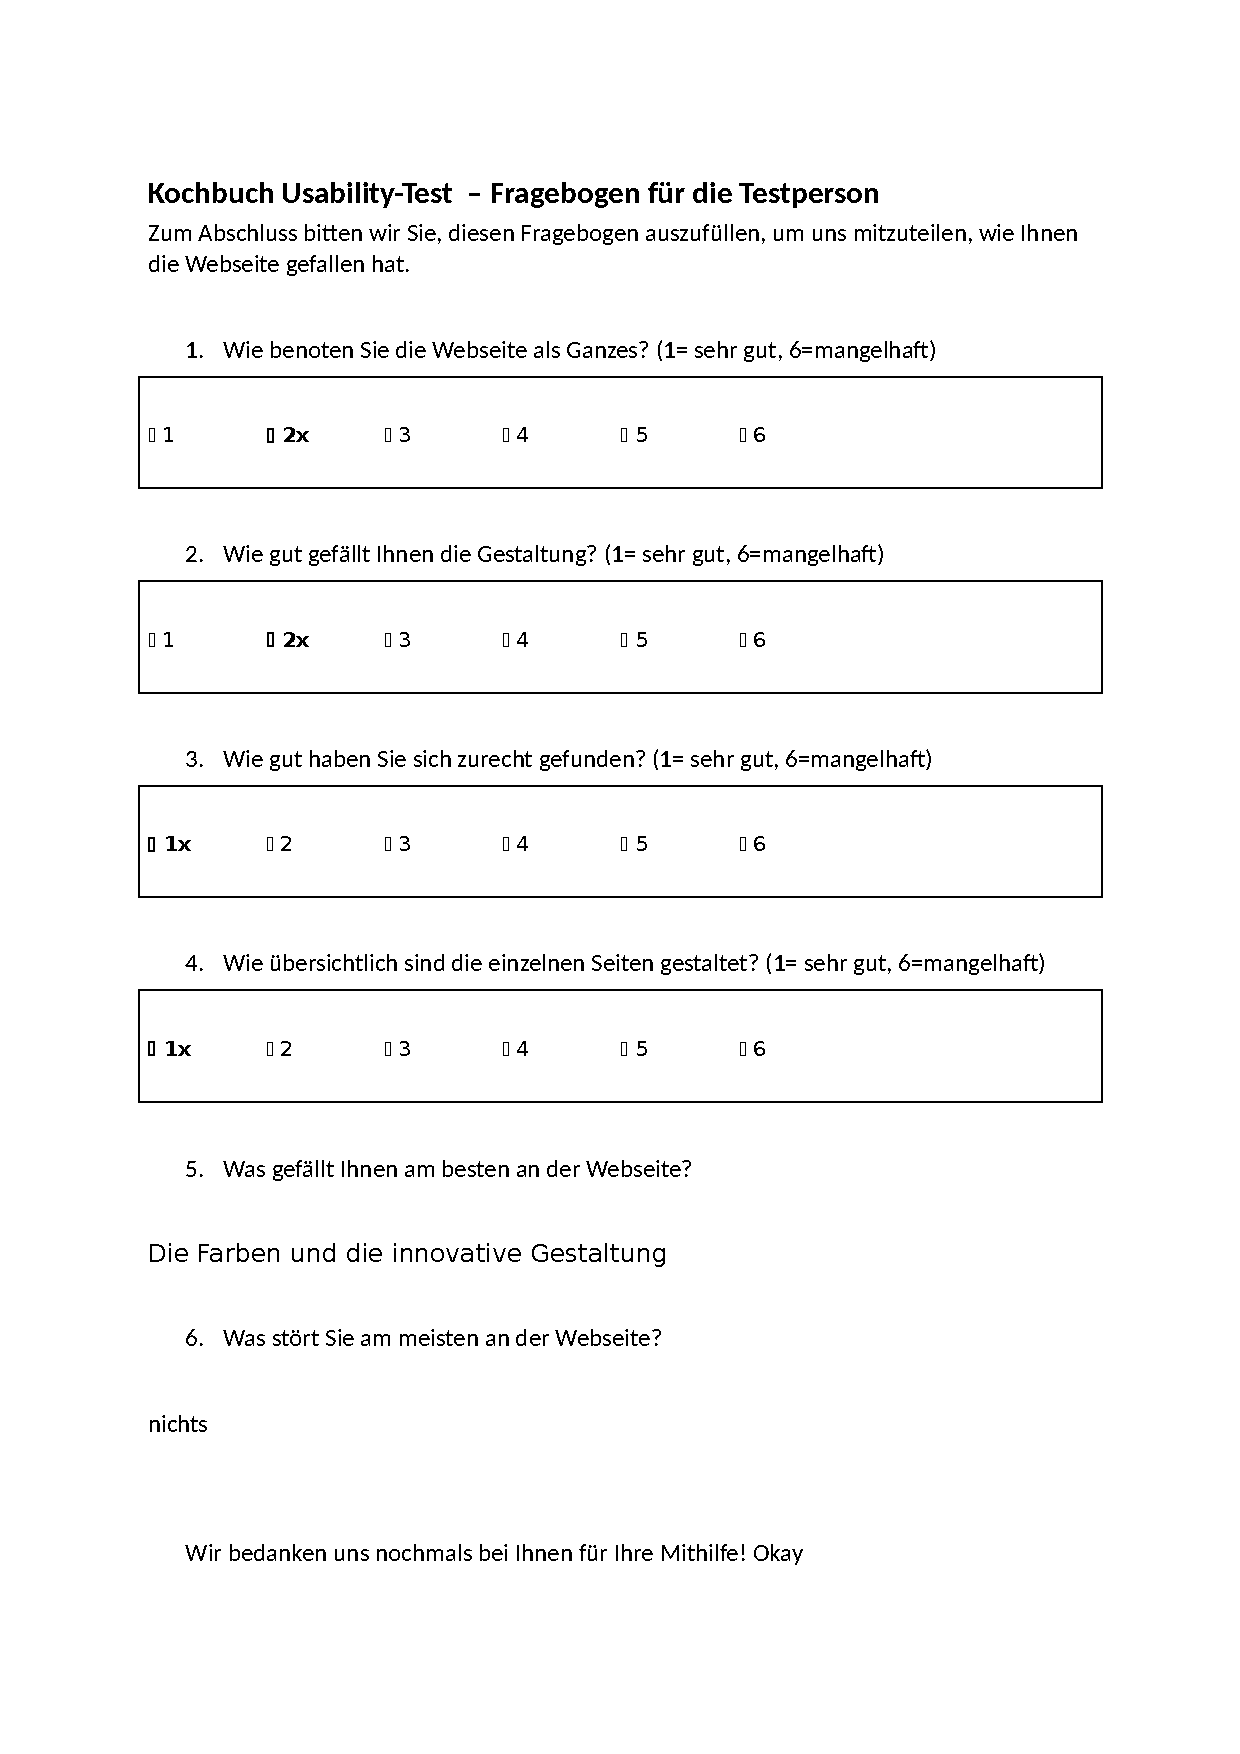
\includegraphics[width=0.8\textwidth]{Fragebogen_Proband3.pdf}
\end{appendix}

\end{document}



